% Adjust these for the path of the theme and its graphics, relative to this file
%\usepackage{beamerthemeFalmouthGamesAcademy}
\usepackage{../../beamerthemeFalmouthGamesAcademy}
\usepackage{multimedia}
\graphicspath{ {../../} }

% Default language for code listings
\lstset{language=C++,
        morekeywords={each,in,nullptr}
}

% For strikethrough effect
\usepackage[normalem]{ulem}
\usepackage{wasysym}

\usepackage{pdfpages}

% http://www.texample.net/tikz/examples/state-machine/
\usetikzlibrary{arrows,automata}

\newcommand{\modulecode}{COMP260}\newcommand{\moduletitle}{Distributed Systems}\newcommand{\sessionnumber}{5}

\begin{document}
\title{\sessionnumber: Optimising for CPU \& Memory}
\subtitle{\modulecode: \moduletitle}

\frame{\titlepage} 

\begin{frame}
	\frametitle{Learning outcomes}
	By the end of today's session, you will be able to:
	\begin{itemize}
		\item \textbf{Understand} the memory hierarchy in modern PC/Consoles/Mobile
		\item \textbf{Implement} optimisations of Data Structures for memory access
		\item \textbf{Describe} CPU Optimisation
	\end{itemize}
\end{frame}

\part{Introduction}
\frame{\partpage}

\begin{frame}
	\begin{itemize}
		\pause \item When we start the optimisation process in games, we want to check if we are CPU or GPU bound
		\pause \item Once this is identified then we can start looking at different ways of optimising our code
		\begin{itemize}
			\pause \item System Level
			\pause \item Algorithm
			\pause \item Micro 
		\end{itemize}
		\pause \item In this session we are going to assume our application is CPU bound 
	\end{itemize}
\end{frame}

\begin{frame}{Optimisation Flow}
	\begin{figure}
		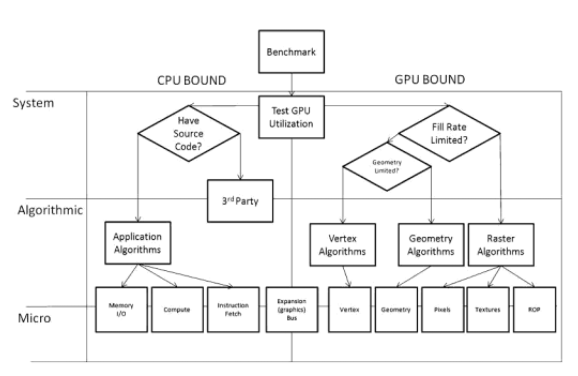
\includegraphics[width=1.0\textwidth,height=0.8\textheight]{OptimisationFlowChart}  
	\end{figure}
\end{frame}
\part{Memory}
\frame{\partpage}

\begin{frame}{Memory Refresher}
	\begin{itemize}
		\pause \item Recall that:
		\begin{itemize}
			\pause \item Dynamic memory, allocated on the \textbf{Heap} and is \textbf{growable}
			\pause \item Static memory, allocated on the \textbf{Stack} and is \textbf{fixed size}
		\end{itemize}
	\end{itemize}
\end{frame}

\begin{frame}{Stack Memory}
	\begin{itemize}
		\pause \item When you allocate value types (int, float, short, char etc), these are allocated on the stack
		\pause \item Values allocated on the stack are local, when they drop out of scope they are deallocated  
		\pause \item Values passed into functions are copied onto the stack
		\pause \item The stack is of fixed size
		\begin{itemize}
			\item C++ Visual Studio - \textbf{1MB}
		\end{itemize}
	\end{itemize}
\end{frame}

\begin{frame}[fragile]{Stack Memory Example 1}
	\begin{lstlisting}
		void Update()
		{
			int x=10;
			int y=10;
	
			Vector2 pos=Vector2(x,y);
		} //<-- x, y and pos drop out of scope here
	\end{lstlisting} 
\end{frame}

\begin{frame}[fragile]{Stack Memory Example 2}
	\begin{lstlisting}[language=C++,basicstyle=\tiny,]
		class MonsterStats
		{
		private:
			int health;
			int strength;
		public:
			MonsterStats()
			{
				health=100;
				strength=10;
			};
	
			void ChangeHealth(int h)
			{
				health+=h;
			};//<- h drops out of scope here
	
			void ChangeStrength(int s)
			{
				strength+=s;
			};//<- s drops out of scope here
		};
	
		void main()
		{		
			//Create an instance of the class on the stack
			MonsterStats stats=MonsterStats();
			stats.ChangeHealth(10);
			stats.ChangeStrength(-2);
		}//<-- stats drops out of scope here
	\end{lstlisting}
\end{frame}

\begin{frame}{Heap Memory}
	\begin{itemize}
	\pause \item Otherwise known as dynamic memory
	\pause \item Types allocated with the \textbf{new} keyword are allocated on the heap
	\pause \item The new operator returns a reference to the type and can be allocated to a pointer (C++)
	\pause \item This heap is managed by the programmer in C++ (see \textbf{delete} keyword) or the garbage collector in C\#
	\pause \item In C++ is very important that you delete anything allocated on the heap
	\pause \item \textbf{for every new, you need a matching delete}
	\pause \item In the Unreal Engine objects can be Garbage Collected
	\end{itemize}
\end{frame}


\begin{frame}[fragile]{Heap Memory Example 1 - C++}
\begin{lstlisting}[language=C++,basicstyle=\tiny,]
	class MonsterStats
	{
	private:
		int health;
		int strength;
	public:
		MonsterStats()
		{
			health=100;
			strength=10;
		}
		
	.....
	}
	
	void main()
	{		
		//Create an instance of the class on the Heap
		MonsterStats * stats=new MonsterStats();
		stats->ChangeHealth(10);
		stats->ChangeStrength(-2);
	
		if (stats)
		{
		delete stats;
		stats=nullptr;
		}
	}
\end{lstlisting}
\end{frame}

\begin{frame}{Passing Variable}
	\begin{itemize}
		\pause \item In C++, we can pass by value or reference. In addition to this, we can also pass in a pointer
		\pause \item We can mark parameter with \textbf{\&} to pass by Reference 
		\pause \item Custom data types and strings should be passed by Pointer or Reference
	\end{itemize}
\end{frame}

\begin{frame}[fragile]{Passing Example 1 - C++}
	\begin{lstlisting}
		int x=10;
	
		void Adder(int &value,int v)
		{
			value+=v;	
		}
	
		Adder(x,10);
		//x would now be 20 after this		
	
	\end{lstlisting}
\end{frame}

\begin{frame}[fragile]{Passing Example 2 - C++}
	\begin{lstlisting}
	
		void SetupMonster(MonsterStats &stats, int health, int strength)
		{
			stats.health=health;
			stats.strength=strength;
		}
		
		//Calling code
		MonsterStats * goblinStats=new MonsterStats();
		SetupMonster(goblinStats,10,2);
	\end{lstlisting}
\end{frame}


\part{CPU}
\frame{\partpage}


\begin{frame}{Further Reading}
	\begin{itemize}
		\item \url{https://software.intel.com/sites/default/files/managed/9e/bc/64-ia-32-architectures-optimization-manual.pdf}
	\end{itemize}
\end{frame}

\end{document}
